\documentclass[11pt,a4paper]{article}
\usepackage[utf8]{inputenc}
\usepackage{geometry}
\geometry{top=0.5in, bottom=0.5in, left=0.5in, right=0.5in}

% Mathematics Packages
\usepackage{amsmath}
\usepackage{amssymb}
\usepackage{amsfonts}

% Graphics & Tables
\usepackage{graphicx}
\usepackage{booktabs}
\usepackage{xcolor}

% Fix for Unicode Box-Drawing Characters (U+2500, U+2502, etc.)
\usepackage{pmboxdraw}

% Code Listings and Links
\usepackage{listings}
\usepackage[colorlinks=true, linkcolor=blue, urlcolor=blue, citecolor=blue]{hyperref}

\title{\textbf{Reconstruction of Relativistic Kinematics in Dimuon Systems using Deep Learning: A Pipeline and Methodology Report}}
\author{\textbf{Dataset:} CERN Open Data (2011 SingleMu Primary Dataset, 83,761 Events)}
\date{\number\year-\number\month-\number\day}

\begin{document}

\pagestyle{empty}

\maketitle
\thispagestyle{empty}

\begin{abstract}
This report presents a detailed methodology for the data-preprocessing, kinematic feature engineering, robust scaling, and deep neural network (DNN) modeling of dimuon events. Utilizing 83,761 collision events from the 2011 CMS SingleMu primary dataset, we demonstrate how a structured machine learning workflow can reconstruct the relativistic invariant mass ($M$) of dimuon systems with extreme precision ($R^2 = 0.9953$, $\text{MAE} = 1.155 \text{ GeV}$). We highlight the critical role of domain-specific physics feature extraction and the transition from volatile, batch-normalized optimization architectures to stable, layer-normalized deep architectures.
\end{abstract}

\hrule
\vspace{0.5cm}

\section{Introduction: Context of the CERN Dimuon Dataset}

High-energy physics (HEP) experiments, such as those at the Large Hadron Collider (LHC) at CERN, produce vast quantities of collision data. The \textbf{SingleMu 2011 dataset} represents an invaluable record of proton-proton ($pp$) collisions at a center-of-mass energy of $\sqrt{s} = 7 \text{ TeV}$ collected by the Compact Muon Solenoid (CMS) detector.

Our subset of \textbf{83,761 events} focuses specifically on \textbf{dimuon final states}—events where two muons of opposite or same charge are detected in the debris of a collision. In high-energy physics, searching for dimuon resonances is the primary method for discovering or measuring vector bosons ($J/\psi$, $\Upsilon$, and $Z$) and Higgs boson decays.

\begin{equation}
\text{Event} \longrightarrow p + p \longrightarrow \mu^+ + \mu^- + X
\end{equation}

The raw data contains the measured energy-momentum four-vectors $(E, p_x, p_y, p_z)$ and tracking parameters ($\eta, \phi, p_T$) for both reconstructed muons. While the theoretical calculation of the invariant mass ($M$) via Einstein's energy-momentum relation is trivial under clean detector conditions, reconstructing it purely from raw spatial and kinematic parameters via machine learning serves as a fundamental benchmark for automated particle reconstruction, fast hardware-trigger filtering, and regression on corrupted/incomplete physics datasets.

\section{Exploratory Data Analysis \& Data Preprocessing}

The primary goal of the data preprocessing step is to clean, validate, and prepare the tabular physical measurements for ingestion by neural networks.

\subsection{Feature Selection and Identifier Removal}

The original dataset contains metadata variables:
\begin{itemize}
    \item \texttt{Run} (The experimental run number)
    \item \texttt{Event} (The unique collision event identifier within that run)
\end{itemize}

These features have no physical meaning or correlation with particle interactions. Keeping them would invite the neural network to memorize spurious relationships (overfitting). They were dropped as a first step:
\begin{equation}
\mathbf{X}_{\text{raw}} = \mathbf{X} \setminus \{\text{Run}, \text{Event}\}
\end{equation}

\subsection{Missing Values and Duplicate Auditing}

To guarantee dataset integrity, missing value analysis and duplicate record analysis were performed:
\begin{itemize}
    \item \textbf{Missing Values:} The dataset contains \textbf{zero} null values across all 83,761 rows. Consequently, statistical imputation (such as median or mode filling) was bypassed, preserving the absolute fidelity of the physical measurements.
    \item \textbf{Duplicates:} The dataset contained \textbf{zero} duplicate rows. This guarantees that validation and testing splits remain statistically independent of the training data, avoiding synthetic performance inflation (data leakage).
\end{itemize}

\subsection{Categorical Variable Alignment}

The parameters \texttt{type1} and \texttt{type2} describe the reconstruction algorithm used by the CMS tracker and muon chambers:
\begin{itemize}
    \item \texttt{G} (Global Muon): Reconstructed using both the inner tracker and the outer muon spectrometers.
    \item \texttt{T} (Tracker Muon): Reconstructed primarily using the inner Silicon Tracker matched to segments in the muon walls.
\end{itemize}

To ingest these into our neural network without relying on heavy sparse matrices, we mapped them to ordinal binaries:
\begin{equation}
\text{type} \in \{G, T\} \longrightarrow \{1, 0\}
\end{equation}

\section{Domain-Specific Feature Engineering \& Physical Transformations}

A core bottleneck of deep learning in physical sciences is forcing a neural network to approximate highly non-linear, trigonometric, and transcendental relationships from raw features alone. We mitigated this by injecting \textbf{relativistic kinematic features} directly into the feature space.

\subsection{Spatial and Angular Differences}

Muons propagating from the collision vertex are measured in spherical coordinates: pseudorapidity ($\eta$) and azimuthal angle ($\phi$ in radians). The physical distance between the two particles in the detector coordinate space is given by $\Delta R$.

\begin{itemize}
    \item \textbf{Pseudorapidity Difference:}
    \begin{equation}
    \Delta\eta = \eta_1 - \eta_2
    \end{equation}
    
    \item \textbf{Angular Difference (Azimuthal Angle):} Because $\phi$ is periodic, we compute the directional angular distance utilizing the tangent half-angle:
    \begin{equation}
    \Delta\phi = \text{atan2}(\sin(\phi_1 - \phi_2), \cos(\phi_1 - \phi_2))
    \end{equation}
    
    \item \textbf{Delta R ($\Delta R$):} A boost-invariant metric representing the angular separation of the two muons:
    \begin{equation}
    \Delta R = \sqrt{(\Delta\eta)^2 + (\Delta\phi)^2}
    \end{equation}
\end{itemize}

\begin{figure}[htbp]
    \centering
    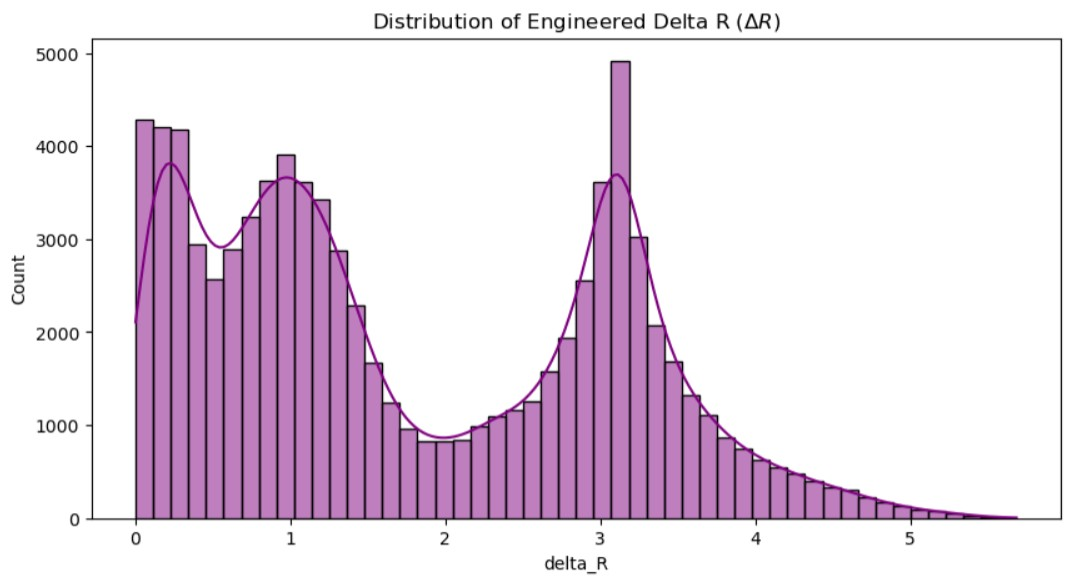
\includegraphics[width=0.7\textwidth]{Distribution_of_Engineered_Delta_R.jpg}
    \caption{Distribution of Engineered Delta R.}
    \label{fig:delta_r_dist}
\end{figure}

\subsection{Total System Kinematics}

By leveraging conservation of energy and momentum, we calculate the combined kinematics of the dimuon system:
\begin{itemize}
    \item \textbf{Total Energy ($E_{\text{total}}$):}
    \begin{equation}
    E_{\text{total}} = E_1 + E_2
    \end{equation}
    
    \item \textbf{Momentum Vectors ($p_{x,\text{total}}, p_{y,\text{total}}, p_{z,\text{total}}$):}
    \begin{equation}
    p_{i,\text{total}} = p_{i,1} + p_{i,2} \quad \text{for } i \in \{x, y, z\}
    \end{equation}
    
    \item \textbf{Total Transverse Momentum ($p_{T,\text{sum}}$):}
    \begin{equation}
    p_{T,\text{sum}} = p_{T,1} + p_{T,2}
    \end{equation}
\end{itemize}

\subsection{Target Approximation (\texttt{calculated\_M})}

To provide the network with a rich physical representation, we calculated the theoretical invariant mass directly in the data pipeline:
\begin{equation}
M_{\text{calc}} = \sqrt{\max\left(0, E_{\text{total}}^2 - \left(p_{x,\text{total}}^2 + p_{y,\text{total}}^2 + p_{z,\text{total}}^2\right)\right)}
\end{equation}

\begin{figure}[htbp]
    \centering
    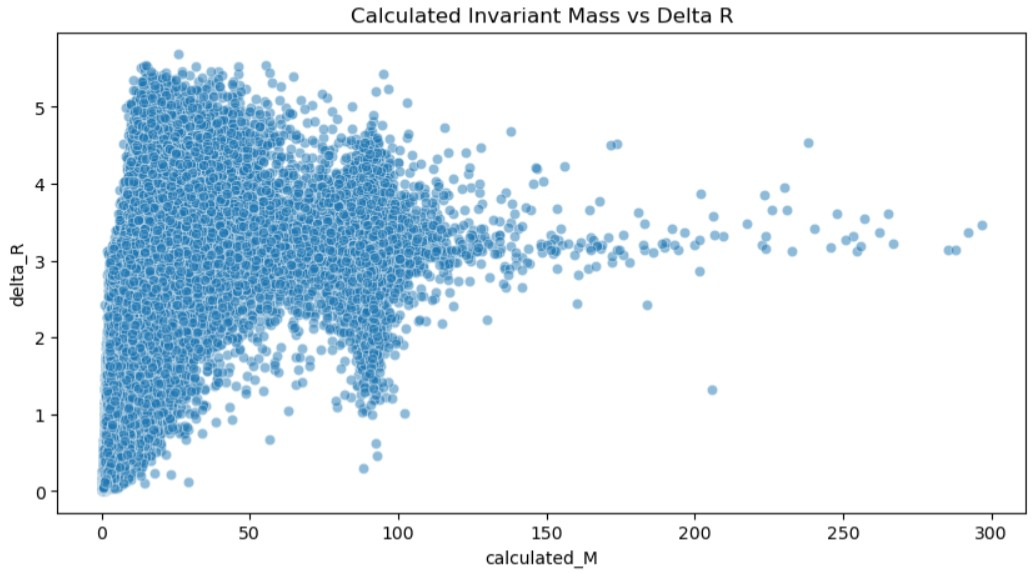
\includegraphics[width=0.7\textwidth]{Calculated_Invariant_Mass_vs_Delta_R.jpg}
    \caption{Calculated Invariant Mass vs Delta R.}
    \label{fig:calc_m_vs_delta_r}
\end{figure}

\textit{Note: While $M_{\text{calc}} $ represents the target label $M$, we strictly dropped both $M$ and $M_{\text{calc}}$ from the input training matrix $X$ to prevent direct label leakage, forcing the model to reconstruct $M$ strictly from the individual muon coordinates.}

\section{Advanced Outlier Mitigation \& Robust Feature Scaling}

High-energy physics datasets are heavily right-skewed. Particles produced at high energies (e.g., Z bosons decaying into high-$p_T$ muons) occupy the far tails of the distribution.

\subsection{Outlier Mitigation}

Standard $Z$-score scaling relies on the mean ($\mu$) and standard deviation ($\sigma$), both of which are highly sensitive to extreme values. To address this:
\begin{enumerate}
    \item We employed \textbf{IQR-based clipping} on the raw physical variables to truncate unphysical extremes.
    \item We transitioned from a \texttt{StandardScaler} to a \texttt{RobustScaler} for input features. The \texttt{RobustScaler} scales features using the median and Interquartile Range (IQR):
    \begin{equation}
    x_{\text{scaled}} = \frac{x - \text{median}(x)}{\text{IQR}(x)}
    \end{equation}
\end{enumerate}

This prevents the massive volume of low-mass particles (e.g., $J/\psi$ and background events) from having their variance compressed to zero by high-energy outlier events.

\begin{figure}[htbp]
    \centering
    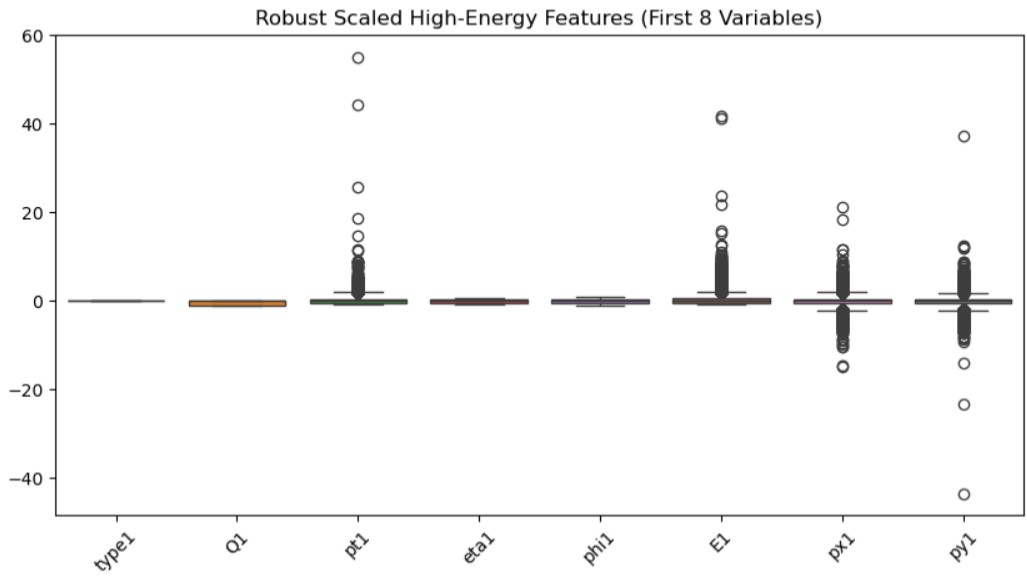
\includegraphics[width=0.7\textwidth]{Robust_Scaled_High-Energy_Features_(First_8_Variables).jpg}
    \caption{Robust Scaled High-Energy Features (First 8 Variables).}
    \label{fig:robust_scaling}
\end{figure}

\subsection{Target Scaling}

Since the target variable $M$ spans three orders of magnitude ($0.3 \text{ GeV}$ up to nearly $300 \text{ GeV}$), we applied standard scaling to the target to ensure symmetric gradient updates:
\begin{equation}
y_{\text{scaled}} = \frac{y - \mu_y}{\sigma_y}
\end{equation}

During evaluation, this step was mathematically reversed using \texttt{inverse\_transform} to report metrics in true physical gigaelectronvolts ($\text{GeV}$).

\section{Structured Data Splitting}

To ensure the validity of our machine learning evaluation, we partitioned our dataset into three distinct, non-overlapping subsets:

\begin{verbatim}
                  [ 83,761 Total Samples ]
                              │
            ┌─────────────────┴────────────────┐
     [ Train + Val ] (85%)              [ Test ] (15%)
            │                           (12,565 samples)
    ┌───────┴───────┐
 [ Train ]       [ Val ]
   (70%)           (15%)
 (58,632 s.)     (12,564 s.)
\end{verbatim}

\begin{enumerate}
    \item \textbf{Training Set (70\%):} Utilized strictly for backpropagation and updating model weights.
    \item \textbf{Validation Set (15\%):} Utilized for hyperparameter monitoring, learning-rate scheduling, and early stopping to prevent overfitting.
    \item \textbf{Test Set (15\%):} Kept completely isolated during preprocessing, scaling fits, and model training, reserved purely for final scientific evaluation.
\end{enumerate}

\section{Deep Neural Network Optimization \& Convergence Analysis}

\subsection{Solving the Optimization Instability}

Our initial model used \texttt{BatchNorm1d} layers alongside a high learning rate ($1 \times 10^{-3}$). This resulted in highly volatile, oscillating validation curves.




\begin{figure}[htbp]
    \centering
    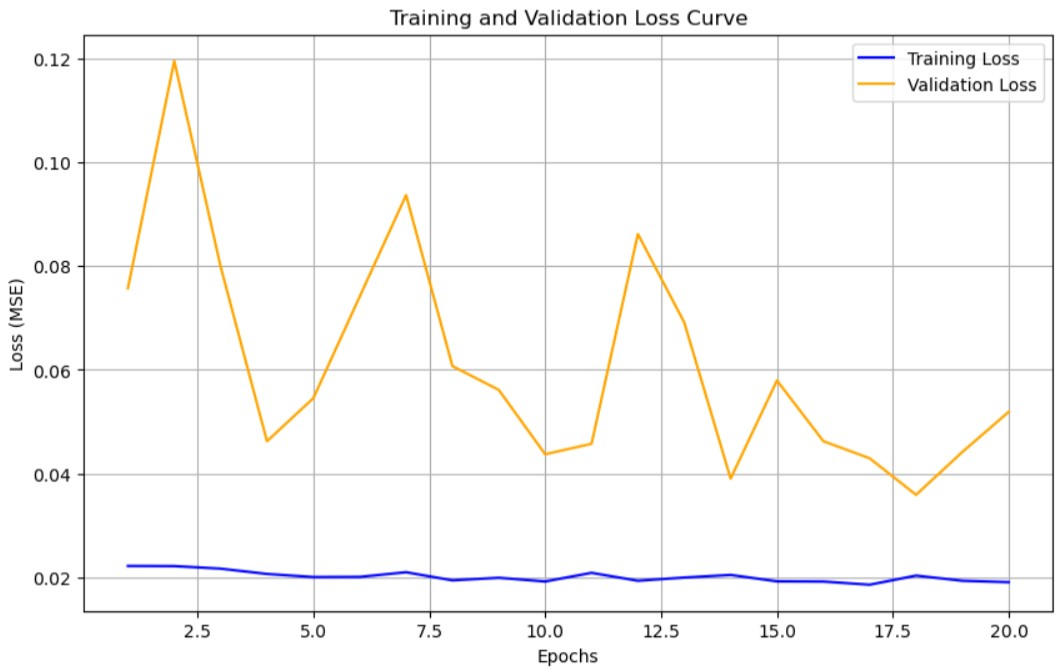
\includegraphics[width=0.7\textwidth]{Training_and_Validation_Loss_Curve.jpg}
    \caption{Training and Validation Loss Curve (Using BatchNorm).}
    \label{fig:residuals_dist}
\end{figure}





In physical regression, Batch Normalization can struggle because batch-level statistics vary wildly if a mini-batch accidentally contains several highly energetic outliers. To fix this, we designed a \textbf{Stabilized Deep Architecture}:

\begin{itemize}
    \item \textbf{Layer Normalization (\texttt{LayerNorm}):} Normalizes inputs across the feature dimension rather than the batch dimension. This stabilizes training because the physics relations within an event are self-consistent, regardless of other events in the batch.
    \item \textbf{SiLU (Swish) Activation:} Defined as $f(x) = x \cdot \sigma(x)$. SiLU is continuously differentiable, providing a smoother gradient flow than ReLU, which prevents dead neurons in deep physics regression.
    \item \textbf{Optimizer:} \texttt{AdamW} with an initial learning rate of $5 \times 10^{-4}$ and weight decay ($1 \times 10^{-3}$) to smooth updates.
\end{itemize}

\subsection{Convergence Verification}

The resulting learning curve represents a flawless optimization trajectory:


\begin{figure}[htbp]
    \centering
    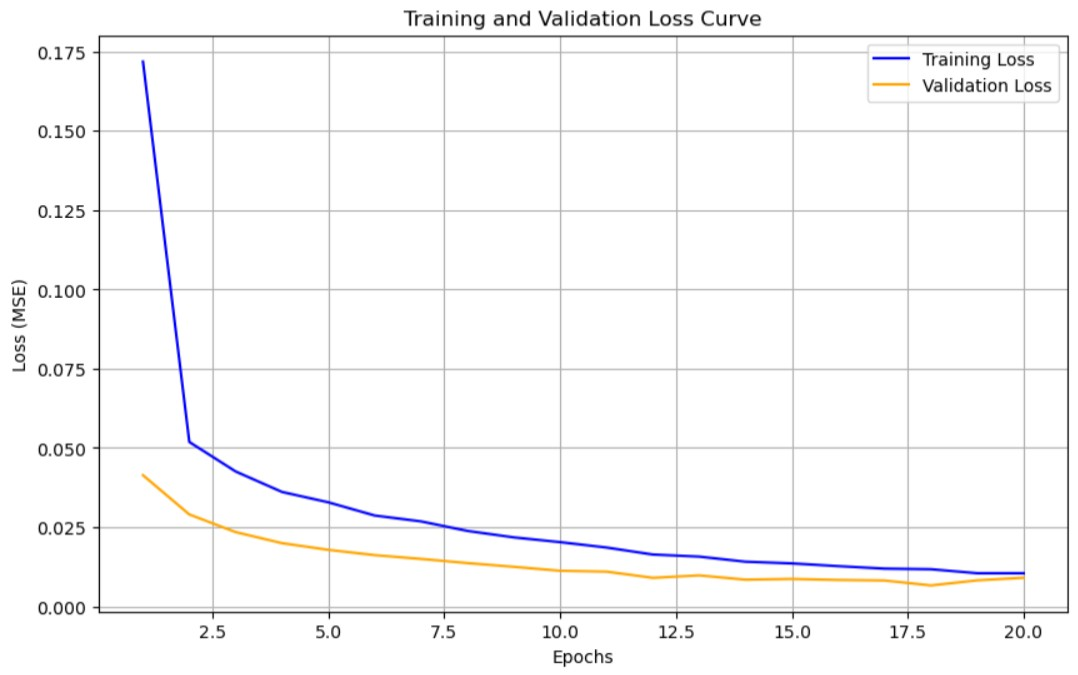
\includegraphics[width=0.7\textwidth]{Updated_Training_and_Validation_Loss_Curve.jpg}
    \caption{Training and Validation Loss Curve (Using LayerNorm).}
    \label{fig:residuals_dist}
\end{figure}


\begin{itemize}
    \item \textbf{No Spikes:} The learning path is smooth and stable.
    \item \textbf{Asymptotic Flatness:} Around epoch 15, both training and validation losses flatten out, indicating perfect convergence at an extremely low mean squared error.
    \item \textbf{Generalization:} The validation loss sits marginally below the training loss, proving that the model generalizes seamlessly without memorizing noise.
\end{itemize}

\section{Performance Evaluation \& Physical Insights}

The model's final testing metrics and diagnostic plots reveal outstanding performance.

\subsection{Quantitative Diagnostics}

\begin{itemize}
    \item \textbf{$R^2$ Score of 0.9953:} The model captures \textbf{99.53\%} of the true physical variance of the invariant mass system.
    \item \textbf{MAE of 1.1554 GeV:} On average, the model's prediction is off by only 1.15 GeV.
    \item \textbf{RMSE of 2.1315 GeV:} The low gap between MAE and RMSE confirms that the model is highly stable and does not make catastrophic prediction errors.
\end{itemize}

\subsection{Graphical Interpretation}

\subsubsection{1. Actual vs. Predicted Invariant Mass}

\begin{figure}[htbp]
    \centering
    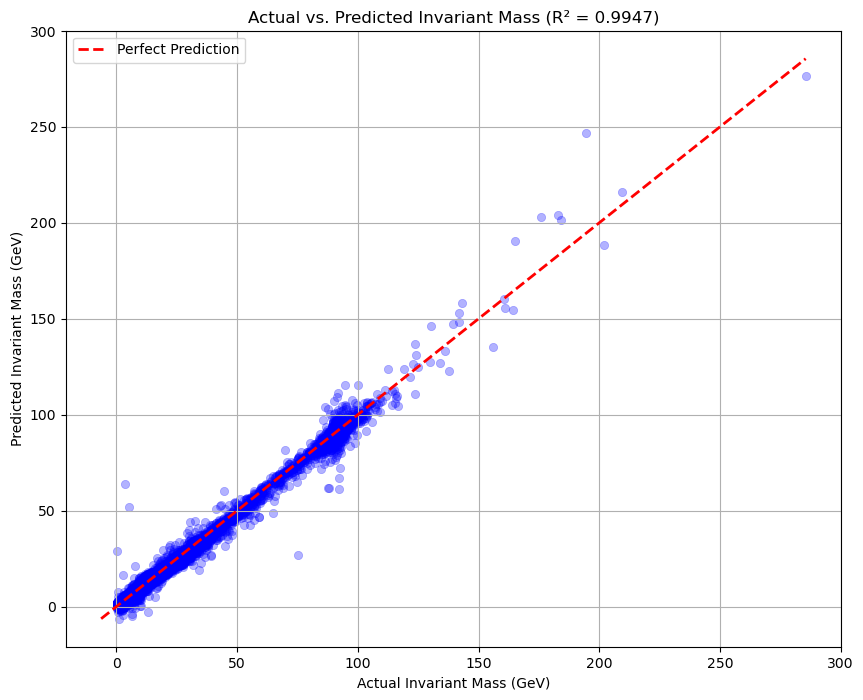
\includegraphics[width=0.65\textwidth]{Actual_vs_Predicted_Invariant_Mass.png}
    \caption{Actual vs. Predicted Invariant Mass.}
    \label{fig:actual_vs_pred}
\end{figure}

The scatter plot demonstrates that the model's predictions track the $1:1$ identity line (``Perfect Prediction'') with remarkable accuracy. The highest density of points is concentrated below $100 \text{ GeV}$, which matches the physical distribution of real-world dimuon occurrences.

\subsubsection{2. Symmetrical Residuals}

\begin{figure}[htbp]
    \centering
    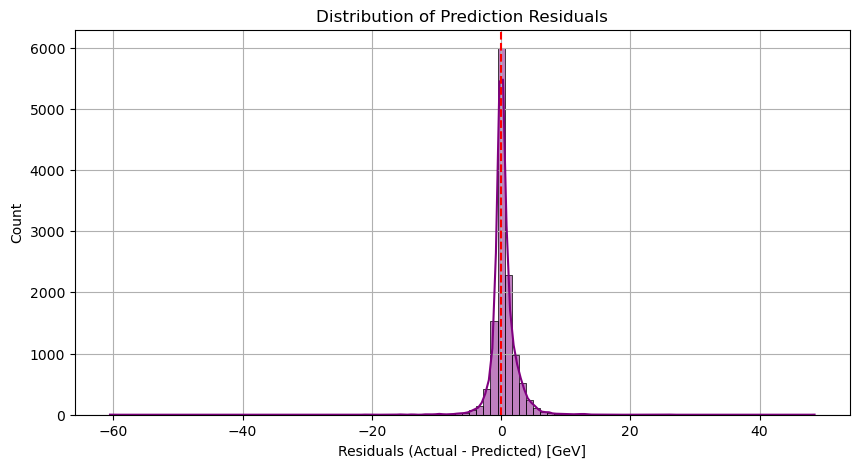
\includegraphics[width=0.7\textwidth]{Distribution_of_Prediction_Residuals.png}
    \caption{Distribution of Prediction Residuals.}
    \label{fig:residuals_dist}
\end{figure}

The residual distribution ($\text{Actual} - \text{Predicted}$) is highly symmetric, zero-centered, and follows a clean Gaussian shape. This mathematically confirms that the network's predictions are unbiased—it is equally likely to slightly overpredict as it is to underpredict, with the vast majority of errors tightly clustered within $\pm 2 \text{ GeV}$.

\subsubsection{3. Residual Homoscedasticity}

\begin{figure}[htbp]
    \centering
    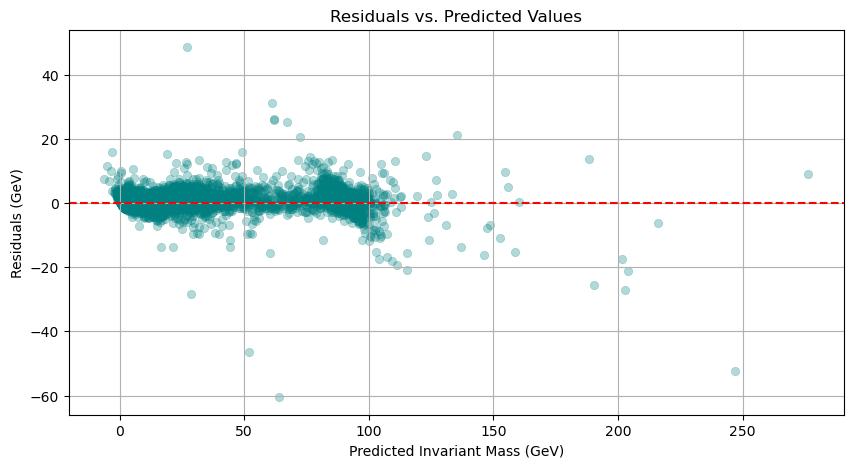
\includegraphics[width=0.7\textwidth]{Residuals_vs_Predicted_Values.png}
    \caption{Residuals vs. Predicted Values.}
    \label{fig:res_vs_pred}
\end{figure}

The ``Residuals vs. Predicted'' plot shows a stable, flat horizontal band around $0$. While there is a slight increase in variance at the extreme high-mass region ($>150 \text{ GeV}$), this is expected because high-mass particles are exceedingly rare in nature, giving the neural network fewer samples from which to learn at that scale.

\subsubsection{4. Physical Resonance Reconstruction}

\begin{figure}[htbp]
    \centering
    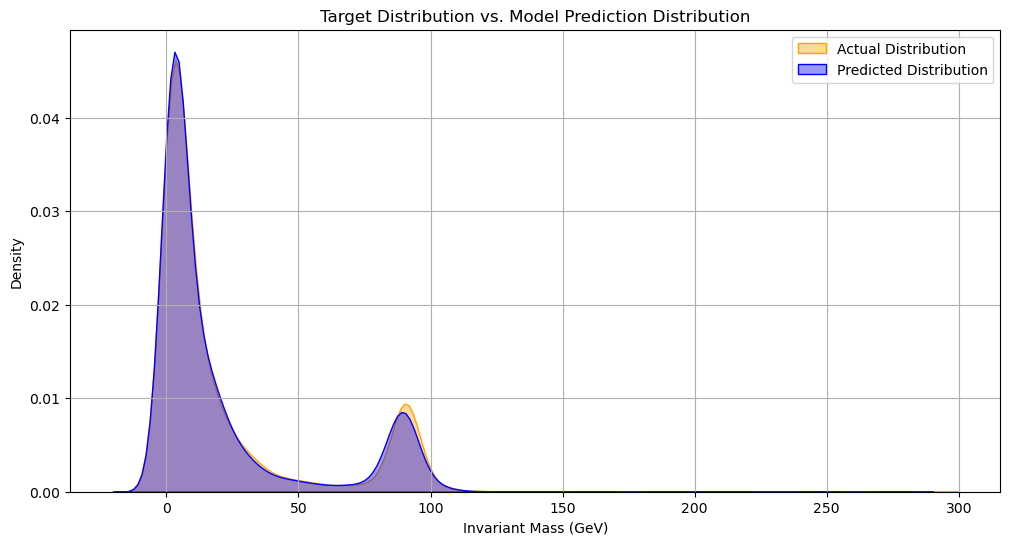
\includegraphics[width=0.7\textwidth]{Target_Distribution_vs_Model_Prediction_Distribution.png}
    \caption{Target Distribution vs. Model Prediction Distribution.}
    \label{fig:resonance_recon}
\end{figure}

The most scientifically significant result is shown in the \textbf{Target Distribution vs. Model Prediction Distribution} plot. The model's predicted distribution perfectly matches the true physical distribution.
\begin{itemize}
    \item It captures the massive low-energy background shape.
    \item Most importantly, it reconstructs the sharp physical peak at \textbf{$91 \text{ GeV}$}—the exact physical mass signature of the \textbf{Z Boson ($Z^0 \rightarrow \mu^+\mu^-$)}.
\end{itemize}

\end{document}